% Essential Formatting

\documentclass[12pt]{article}
\usepackage{epsfig,amsmath,amsthm,amssymb}
%\usepackage[questions, answersheet]{urmathtest}[2001/05/12]
%\usepackage[answersheet]{urmathtest}[2001/05/12]
\usepackage[answers]{urmathtest}[2001/05/12]


% For use with pdflatex
% \pdfpagewidth\paperwidth
% \pdfpageheight\paperheight

% Basic User Defs

\def\ds{\displaystyle}

\newcommand{\ansbox}[1]
{\work{
  \pos\hfill \framebox[#1][l]{ANSWER:\rule[-.3in]{0in}{.7in}}
}{}}

\newcommand{\ansrectangle}
{\work{
  \pos\hfill \framebox[6in][l]{ANSWER:\rule[-.3in]{0in}{.7in}}
}{}}


% Beginning of the Document

\begin{document}
\examtitle{LINEAR REGRESSION MODELS W4315}{HOMEWORK 2}{09/16/2009}
 \begin{center}
  Instructor: Frank Wood
 \end{center}
%%\studentinfo
\instructions{
  %\textbf{Circle your Instructor's Name along with the Lecture Time:}



  \begin{itemize}
  \item
    \textbf{Please show all your work.
            You may use back pages if necessary.}
  %\item
   % \textbf{Please put your \underline{simplified}
   %         final answers in the spaces provided.}
  \end{itemize}
}
\finishfirstpage

% Problems Start Here % ----------------------------------------------------- %


\problem{20} {
 In the file "problem1.txt"(accessible on professor's website),
 there are 500 pairs of data, where the first column is X and
 the second column is Y. The regression model is
 $Y=\beta_0+\beta_1X+\epsilon$\\
 a. Draw 20 pairs of data randomly from this population of size 500.
 Use MATLAB to run a regression model specified as above and keep
 record of the estimations of both $\beta_0$ and $\beta_1$. Do this
 200 times. Thus you will have 200 estimates of $\beta_0$ and $\beta_1$.
 For each parameter, plot a histogram of the estimations.\\
 b. The above 500 data are actually generated by the model
 $Y=3+1.5X+\epsilon$, where $\epsilon\sim N(0,2^2)$. What is the
 exact distribution of the estimates of $\beta_0$ and $\beta_1$?\\
 c. Superimpose the curve of the estimates' density functions from
 part b. onto the two histograms respectively. Is the histogram a
 close approximation of the curve?
   }
 { \vfill
  \answer
} {First, read the data into Matlab.\\
pr1=textread('problem1.txt');\\
V1=pr1(1:250,1);\\
V2=pr1(1:250,2);\\
T1=pr1(251:500,1);\\
T2=pr1(251:500,2);\\
X=[V1;V2];\\
Y=[T1;T2];\\
Randomly draw  20 pairs of (X,Y) from the original data set, calculate the coefficients $b_0 $ and $b_1 $ and repeat the process  for 200 times\\
b0=zeros(200,1);\\
b1=zeros(200,1);\\
i=0\\
for i=1:200\\
indx=randsample(500,20);\\
x=X(indx);\\
y=Y(indx);\\
$avg\_x = mean(x);$\\
$avg\_y = mean(y);$\\
$sxx= sum((x-avg\_x).^2);$\\
$sxy= sum((x-avg\_x).*(y-avg\_y));$\\
$b1(i) = sxy/sxx;$\\
$b0(i) = avg\_y-b1(i)*avg\_x;$\\
end;\\
Draw histograms of the coefficients $b_0$ and $ b_1$\\
hist(b0)\\
hist(b1)\\
\begin{figure}[h!]
\centering
\graphicspath{{c:/users/qun/desktop/}}
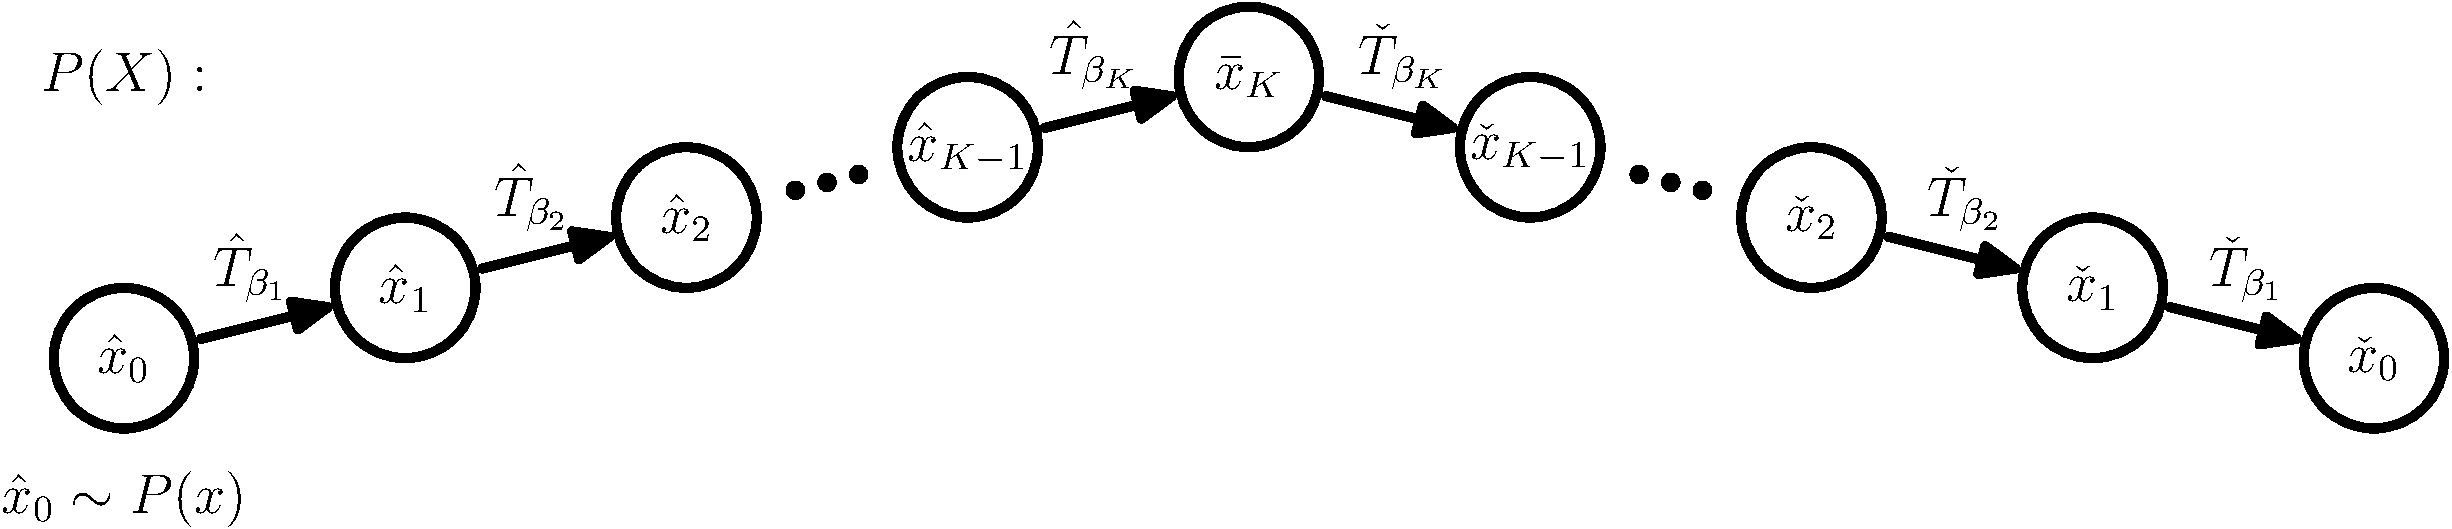
\includegraphics[scale=.5]{figure1.png}
\caption{Histogram of $b_0$}
\end{figure}

\begin{figure}[h!]
\centering
\graphicspath{{c:/users/qun/desktop/}}
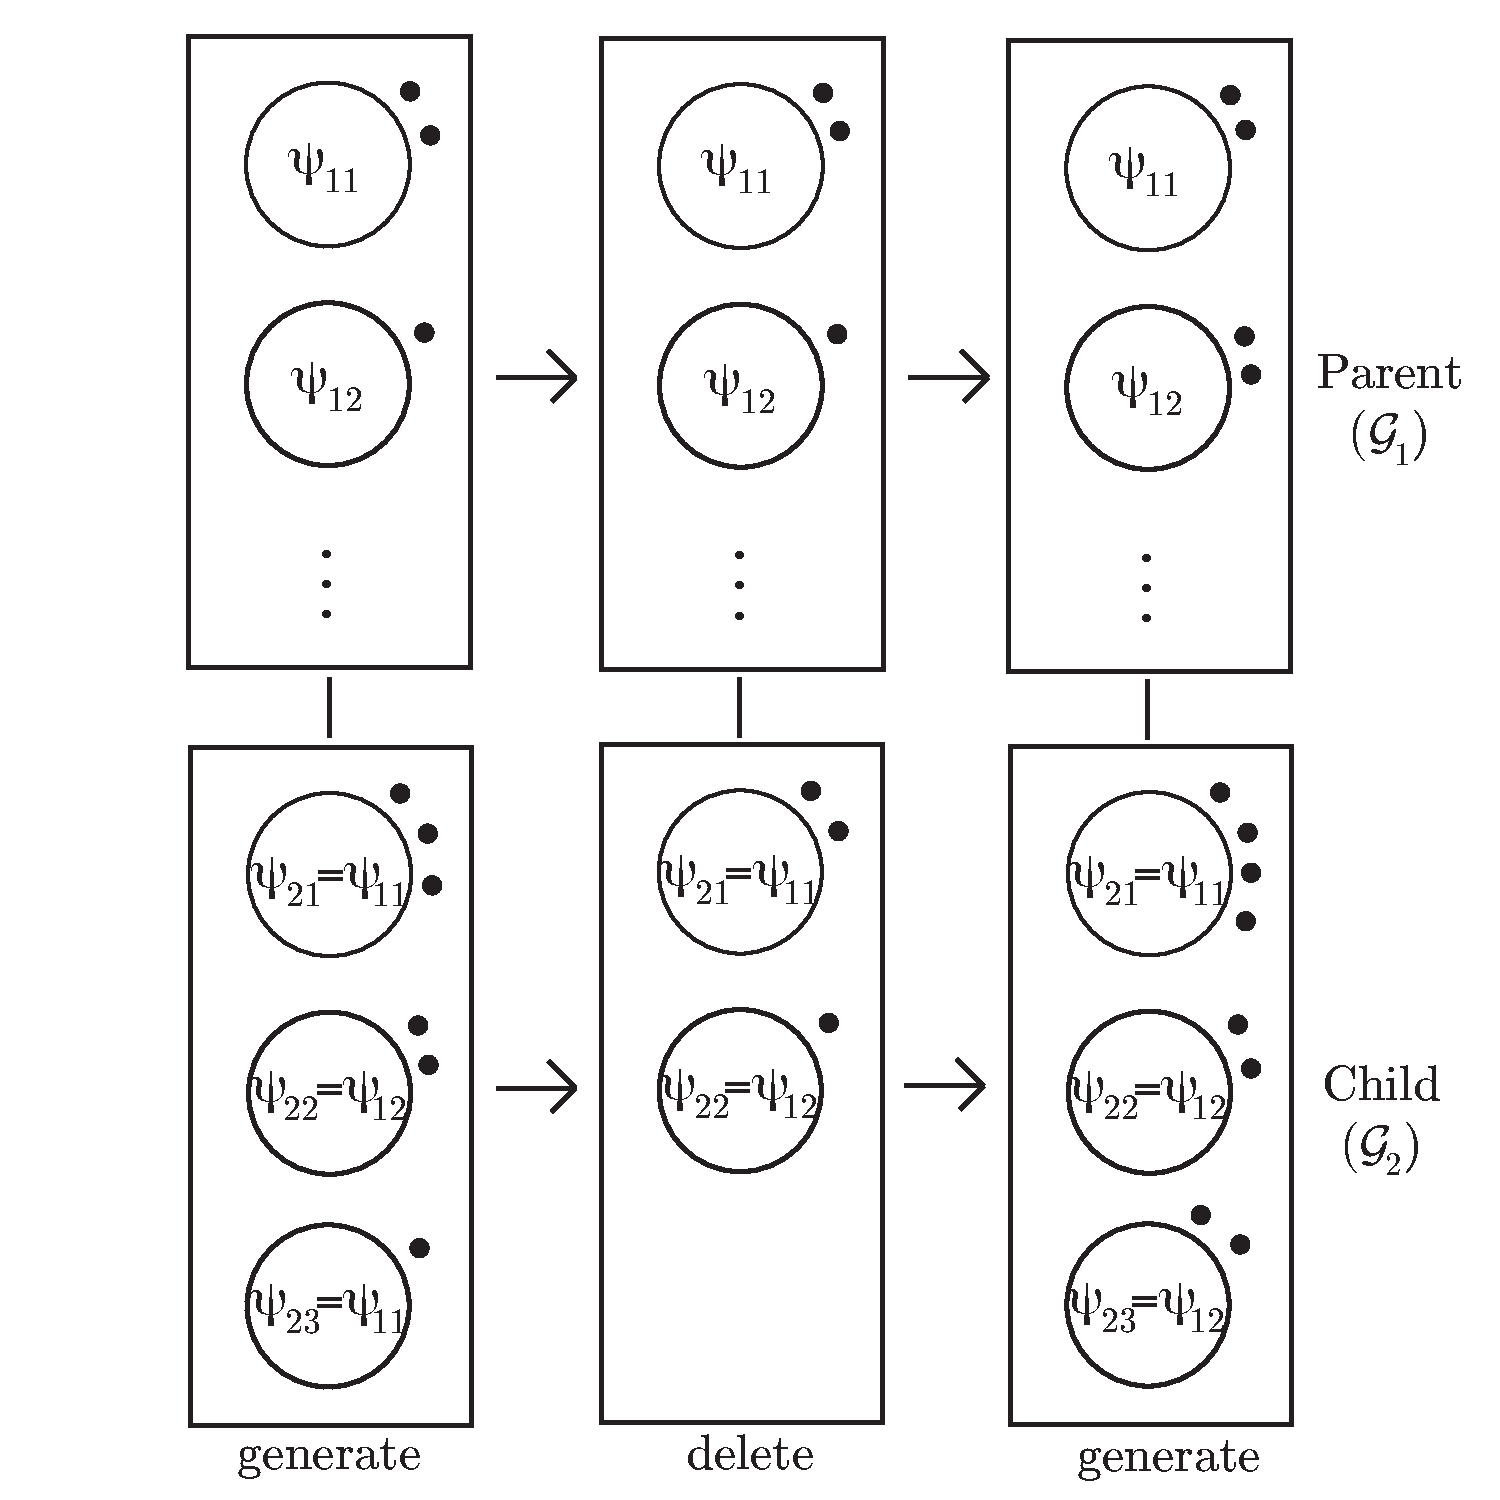
\includegraphics[scale=.4]{figure2.png}
\caption{Histogram of b1}
\end{figure}

b. As we have known,
$b_1 = \frac{\sum_i(X_i-\bar X)(Y_i - \bar Y)}{\sum_i(X_i-\bar X)^2}=\frac{\sum_i(X_i-\bar X)Y_i}{\sum_i(X_i-\bar X)^2}=\sum_i K_iY_i$     where$ K_i=\frac{X_i-\bar X}{\sum_i(X_i-\bar X)^2}$
So, $b_1$ is a linear combination of $Y_i$. Since $Y_i$ has a normal distribution, $ b_1$ also follows a normal distribution.\\
$E(b_1)=\sum_i K_iE(Y_i)=\sum_i K_i(\beta_0+\beta_1X_i)=\sum_i K_i\beta_0 +(\sum_i K_iX_i )\beta_1$\\
$\sum_i K_i=\frac{\sum_i(X_i-\bar X)}{\sum_i(X_i-\bar X)^2}=0$\\
$\sum_i K_iX_i=\frac{\sum_i(X_i-\bar X)X_i}{\sum_i(X_i-\bar X)^2}=\frac{\sum_i(X_i-\bar X)(X_i-\bar X)}{\sum_i(X_i-\bar X)^2}=1$\\
 $E(b_1)=0+1*\beta_1=\beta_1$\\
$Var(b_1)=\frac{\sigma^2}{\sum_i(X_i-\bar X)^2}$ (see the proof in homework 1 solution)\\
Therefore, $ b_1\sim N(\beta_1,\frac{\sigma^2}{\sum_i(X_i-\bar X)^2})$\\
$b_0 = \bar Y - b_1 \bar X$\\
$E(b_0)=\beta_0$\\
$Var(b_0)=(\frac{1}{n}+\frac{\sum{X_i}^2}{\sum_i(X_i-\bar X)^2})\sigma^2$\\
Therefore,  $ b_0 \sim N(\beta_0,(\frac{1}{n}+\frac{\sum{X_i}^2}{\sum_i(X_i-\bar X)^2})\sigma^2)$\\
Since the  data are  generated by the model
 $Y=3+1.5X+\epsilon$, where $\epsilon\sim N(0,2^2)$.\\
 $\beta_0=3; \beta_1=1.5 $ and $\sigma^2=4$.
The mean and variance of $b_0$ and $b_1$ can thus be determined. 
Calculate the variance of $b_0$ and $b_1$ in Matlab\\
$avg\_X= mean(X);$\\
avg\_Y = mean(Y);\\
$SXX = sum((X-avg\_X).^2);$\\
$SXY = sum((X-avg\_X).*(Y-avg\_Y));$\\
$B1 = SXY/SXX;$\\
B0 = avg\_Y - b1*avg\_X;\\
% calculate the variance of bo and b1
var\_B1=4/SXX\\
$var\_B0=4*(1/500+((avg\_X).^2)/SXX)$\\
$sd\_B0=sqrt(var\_B0)$\\
$sd\_B1=sqrt(var\_B1)$\\
The results showed that $Var(b_0)=0.0334$; $Var(b_1)=9.457E-004$\\
 The exact distribution of the estimates of $\beta_0$ and $\beta_1$ is 
$b_0 \sim  N(3,0.0334); b_1 \sim N(1.5,9.457E-004)$

c. We have obtained the estimates' exact distribution in part(b), we can now plot the curve of their pdf function and compare them with the histograms. 

$a = 0:0.1:6;$\\
$mu = 3;$\\
$sigma =sd\_B0$;\\
pdfNormal = normpdf(a, mu, sigma);\\
$[n,xout]=hist(b0);$\\
$n=6*n/200;$\\
bar(xout,n)\\
hold on;\\
plot(a, pdfNormal)\\
hold off\\
xlabel('b0')\\
ylabel('6*Frequency')\\

\begin{figure}[h!]
\centering
\graphicspath{{c:/users/qun/desktop/}}

\includegraphics[scale=.6]{figure3.png}
\caption{Histogram and the pdf curve of $b_0$ on the same plot}
\end{figure}

$b=1:0.1:2$\\
$mu=1.5;$\\
$sigma=sd\_B1;$\\
pdfNormal = normpdf(b, mu, sigma);\\
$[n,xout]=hist(b1);$\\
$n=40*n/200;$\\
bar(xout,n)\\
hold on;\\
plot(b, pdfNormal)\\
hold off\\
xlabel('b1')\\
ylabel('40*Frequency')\\

\begin{figure}[h]
\centering
\graphicspath{{c:/users/qun/desktop/}}
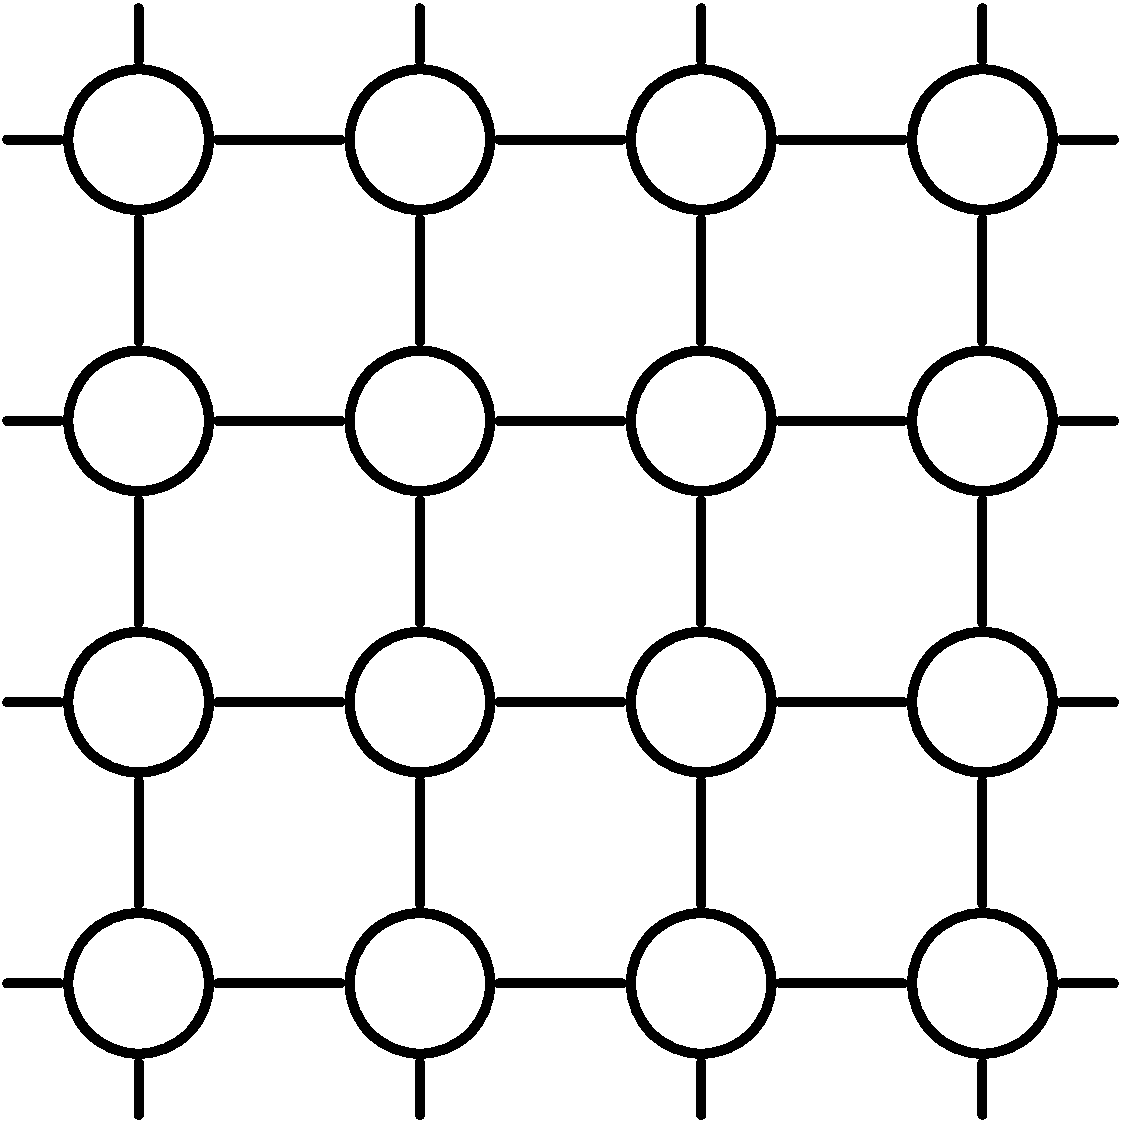
\includegraphics[scale=.6]{figure4.png}
\caption{Histogram and pdf curve of$ b_1$ on the same plot}
\end{figure}
As we can see from Figure 3 and Figure 4, the shape of the histogram of the coefficients obtained from the 200 times simulations is similar to that of the curve of the estimated distubtioin of the coefficients. 
}




\problem{20} {
 Use the same data set in the last problem, we will estimate
 $\beta_0$ and $\beta_1$ using Newton-Raphson method.\\
 a. Draw a 3d plot using MATLAB(check "surf" command for example) to
 illustrate how the SSE varies according to different combinations
 of estimates of $\beta_0$ and $\beta_1$. So to speak, draw a 3d
 plot where x and y axes represent different values of slope and
 intercept of the regression line respectively, while z axis is the
 SSE.\\
 b. Use Newton-Raphson method to minimize the SSE and give estimates
 of the parameters(slope and intercept) of the regression line. Give
 a geometrical interpretation of the method and explain how it
 works.
  }
 { \vfill
  \answer
} { 
a. Use the" surf" command in Matlab to draw the 3D plot 

$z=zeros(61,61);$\\
$x=[0:0.1:6];$\\
$y=[-1.5:0.1:4.5];$\\
$i=0;$\\
$j=0;$\\
for i=1:61\\
    for j=1:61\\
    $z(i,j)=sum((Y-x(j)-y(i)*X).^2);$\\
    end\\
end\\
meshgrid(x,y,z)\\
surf(x,y,z)\\
\begin{figure}[h!]
\centering
\graphicspath{{c:/users/qun/desktop/}}
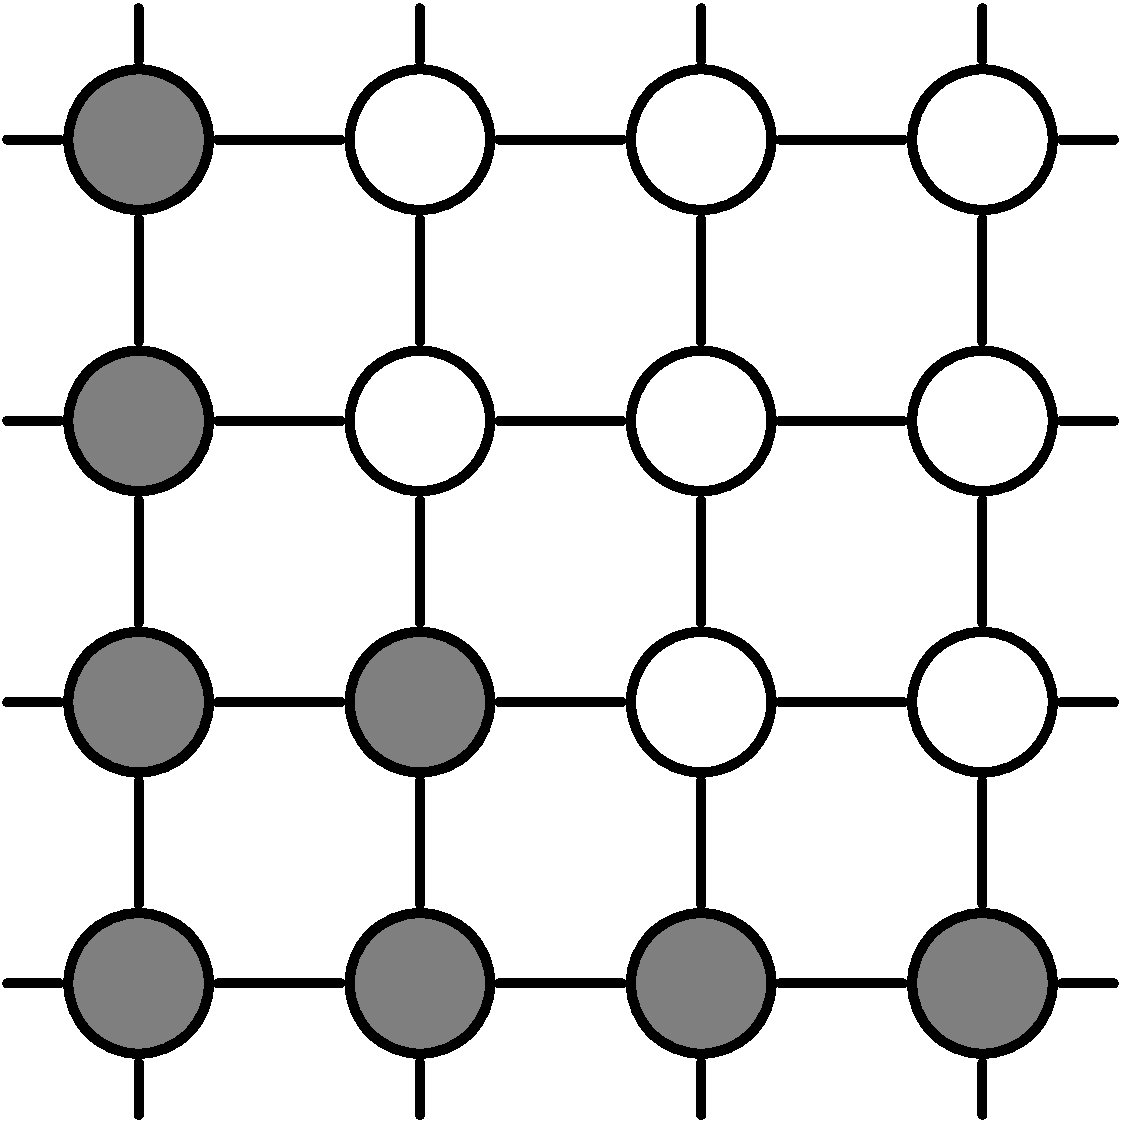
\includegraphics[scale=.6]{figure5.png}
\caption{3D plot of SSE versus the slope and the intercept of the regression line }
\end{figure}

 b. Use Newton-Raphson method to minimize the function $F(\beta)=SSE$ and get the estimates of the parameters. Here we use the iterations $H_F(\beta_n)(\beta_{n+1}-\beta_n)=\nabla F(\beta_n)$\\
where $H_F(\beta_n)$ is the Hessian matrix(second-order partial derivatives of the function SSE) and$\nabla F(\beta_n)$ is gradient.\\
$\nabla F= \begin{bmatrix} -2\sum_i(Y_i-\beta_0-\beta_1 X_i) \\
 -2\sum_i ((Y_i-\beta_0-\beta_1 X_i)X_i) \end{bmatrix}$
$H_F= \begin{bmatrix} 2n& 2\sum_i X_i\\
2\sum_i X_i & 2\sum_i(X_i^2) \end{bmatrix}$
$\beta=\begin{bmatrix}\beta_0\\
\beta_1\end{bmatrix}$\\
 
The Matlab code is:\\
function[beta,SSE]= NR\_linear(data,beta\_start)\\
$x=data(:,1);$\\
$y=data(:,2);$\\
$n=length(x);$\\
diff=1;beta=beta\_start;\\
while diff$> 0.0001$\\
   beta\_old=beta;\\
    J=[-2*sum(y-beta(1)-beta(2)*x);-2*sum((y-beta(1)-beta(2)*x).*x)]\\     
   $ H=[2*n, 2*sum(x); 2*sum(x), 2*sum(x.^2)]$\\
    H\_1=inv(H);\\
   $SSE=sum((y-beta(1)-beta(2)*x.^2)$\\
   beta=beta\_old - H\_1*J\\
    diff=sum(abs(beta - beta\_old));\\
end\\
hw1=[X,Y]\\
beta0=[0;0]\\
$[betaml,sse] = NR\_linear(hw1,beta0)$\\
Using Newton Ralphson method, we got the same result with the least square method, $b_0=2.7725$ $b_1=1.5297.$\\
The geometric interpretation of Newton's method is that at each iteration one approximates  by a quadratic function around F(x), and then takes a step towards the maximum/minimum of that quadratic function.
}

\problem{10} {
 a. In simple linear regression setting $y=\beta_0+\beta_1x+\epsilon$, write out the explicit form the error function.\\
 b. Prove this function is convex with respect to its variables($\beta_0$ and $\beta_1$). }
 { \vfill
  \answer
} {
The error function$ E=\sum_{i=1}^n(Y_i-\beta_0-\beta_1*X_i)^2$\\
To prove the error function is convex with respect to $\beta_0$ and $\beta_1$, we need to show that the Hessian matrix of the error function is postive- semidefinite.\\
Suppose we have a non zero vector $Z=\begin{bmatrix}z_1\\
z_2\end{bmatrix}$\\
$Z^THZ=\begin{bmatrix}z_1&z_2\end{bmatrix}\begin{bmatrix}2n& 2\sum_i X_i\\
2\sum_i X_i & 2\sum_i(X_i^2) \end{bmatrix}\begin{bmatrix}z_1\\
z_2\end{bmatrix}=\begin{bmatrix}2nz_1+2z_2\sum_iX_i & 2z_1\sum_iX_i+2z_2\sum_iX_i^2\end{bmatrix}\begin{bmatrix}z_1\\
z_2\end{bmatrix}$\\
$=2nz_1^2+4z_1z_2\sum_iX_i+2z_2^2\sum_iX_i^2$\\
$=2[nz_1^2+2z_1z_2\sum_iX_i+z_2^2\sum_iX_i^2]$\\
$=2[(z_1+X_iz_2)^2]\geq0$ for any non zero vector $Z\in R^n$\\
The Hessian Matrix of the error function with respect to $\beta_0$ and $\beta_1$ is postive-semidefinite and therefore the error function is a convex function.

}



% Problems End Here % ------------------------------------------------------- %

\problemsdone
\end{document}

% End of the Document
